\documentclass{beamer}

\usepackage{amsmath}
\usepackage{amssymb}
\usepackage{tikz}
\usepackage{pgfplots}

\title{Orthogonality}
\subtitle{The ``Whole" of Chapter 6}
\author{Ahmed Mohammed}
\institute{Georgia Institute of Technology}
\date{PLUS Session, Summer 2023}

\usetheme{Copenhagen}
\usefonttheme{serif}
\usecolortheme{seagull}

\renewcommand{\vec}[1]{\mathbf{#1}}

\AtBeginSection[]
{
    \begin{frame}
        \frametitle{Table of Contents}
        \tableofcontents[currentsection]
    \end{frame}
} % https://statisticaloddsandends.wordpress.com/2019/02/18/beamer-inserting-section-slides-before-each-section/

\begin{document}
	\begin{frame}
		\maketitle
	\end{frame}

	\section{Open Activity: Quick Introductions}
	% Leave three questions for each subsection. Students should be familiar enough, so I'll just skip to questions quickly. ~10 minutes.
	\subsection{6.1 \& 6.2}
	\begin{frame}
		\frametitle{The Dot Product and Length}
		\(\forall \vec{v}, \vec{u} \in \mathbb{R}^n,\)
		\begin{itemize}
			\item<2-> \(\vec{v} \cdot \vec{u} = \vec{v}^{T}\vec{u} = v_1u_1 + v_2u_2 + \dots + v_nu_n\);
			\item<3-> \(\vec{v} \cdot \vec{v} = \|\vec{v}\|^2\);
			\item<4-> \(\vec{v} \perp \vec{u} \iff \vec{v} \cdot \vec{u} = 0\);
			\item<5-> \(d(\vec{v}, \vec{u}) = \|\vec{v} - \vec{u}\|\);
			\item<6-> \textit{Distance between a subspace and a vector will be discussed later}.
		\end{itemize}
	\end{frame}

	\begin{frame}
		\frametitle{Orthogonal Complements}
		\begin{itemize}
			\item<1-> If we have a subspace \(W\) of \(V\), a vector \(\vec{v}\), and \(\forall \vec{u} \in W \), \(\vec{v} \perp \vec{u},\) then \(\vec{v}\) is
				\emph{orthogonal} to \(W\).

				\only<1>{\begin{figure}[!h]
					\centering
					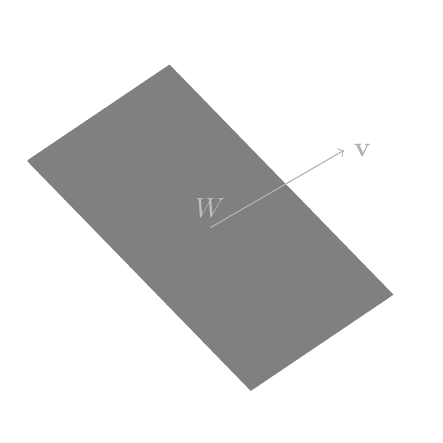
\begin{tikzpicture}
						\begin{axis}
								[height=6.5cm, width=6.5cm,
								 view={30}{25}, axis line style = {draw=none}, tick style = {draw=none}, 
								 xtick=\empty, ytick=\empty, ztick=\empty]
							\addplot3[shader=flat, surf, gray] {-x} node[pos=0.5, above]{\color{gray!50!white}\(W\)};
							\addplot3[->, gray!60!white] coordinates {(0, 0, 0) (6, 0, 6)} node[right] {\(\vec{v}\)};
						\end{axis}
					\end{tikzpicture}
				\end{figure}
				}

			\item<2-> If we have a subspace \(W\) of \(V\), the set of all vectors that are orthogonal to it is called the orthogonal complement, 
					\(W^\perp\).

				\only<2>{\begin{figure}[!h]
					\centering
					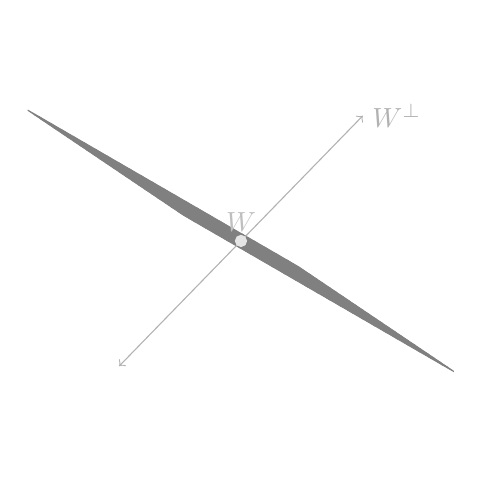
\begin{tikzpicture}
						\begin{axis}
								[height=7cm, width=7cm,
								 view={330}{25}, axis line style = {draw=none}, tick style = {draw=none}, 
								 xtick=\empty, ytick=\empty, ztick=\empty]
							\addplot3[shader=flat, surf, gray] {-x} node[pos=0.5, above]{\color{gray!50!white}\(W\)};
							\addplot3[<->, domain=-4.5:4.5, gray!60!white] ({x}, {0}, {x}) node[right] {\(W^\perp\)};
							\addplot3[mark=*, gray!20!white] coordinates {(0, 0, 0)};
						\end{axis}
					\end{tikzpicture}
				\end{figure}
				}

			\item<3-> Note that \(\dim W + \dim W^\perp = \dim V\).
		\end{itemize}
	\end{frame}

	\subsection{6.3}
	\begin{frame}
		\frametitle{Orthogonal Projections \& Decompositions}
		\begin{enumerate}
			\item<1-> Every vector in \(\mathbb{R}^n\) can be \emph{uniquely} decomposed into the sum of two vectors, \(\vec{\hat{y}} \in W\) and \(\vec{y}_{\perp} \in W^\perp\).
			\item<2-> \(\vec{\hat{y}}\) is called the orthogonal projection of \(\vec{y}\) onto \(W\), denoted as \(\operatorname{proj}_{W}\vec{y}\).
			\item<3-> If \(\{\vec{u}_1, \vec{u}_2, \dots, \vec{u}_p\}\) is an \emph{orthonormal} basis for \(W\), and \(U = \begin{bmatrix}\vec{u}_1 & \cdots & \vec{u}_p\end{bmatrix},\) then \[\operatorname{proj}_W \vec{y} = UU^T \vec{y}.\]
		\end{enumerate}
	\end{frame}

	\begin{frame}
		\frametitle{Theorem: The Best Approximation Theorem}

		\begin{theorem}
			If \(W \subset \mathbb{R}^{n}\), and \(\vec{y} \in \mathbb{R}^n\), then 
			\[\|\operatorname{proj}_W\vec{y} - \vec{y} \| < \|\vec{w} - \vec{y}\|\]
			for any \(\vec{w} \in W\) with \(\vec{w} \ne \operatorname{proj}_W\vec{y}.\)
		\end{theorem}

	\end{frame}

	\section{Main Activity: Exercises}
	\begin{frame}
		\frametitle{Practice Problems}
		Look at worksheet.
	\end{frame}

	\section{Closing Activity: 'Till Next Time}
	\begin{frame}
		We'll be reviewing for the exam next session! \pause

		Gram-Schmidt and least-square solutions.
	\end{frame}
	
\end{document}
